\documentclass{article}
\setlength{\oddsidemargin}{0.25 in}
\setlength{\evensidemargin}{-0.25 in}
\setlength{\topmargin}{-0.6 in}
\setlength{\textwidth}{6.5 in}
\setlength{\textheight}{8.5 in}
\setlength{\headsep}{0.75 in}
\setlength{\parindent}{0 in}
\setlength{\parskip}{0.1 in}

% ===== PACKAGES =====
\usepackage{amsmath,amssymb}
\usepackage{color}
\usepackage{subfigure}
\usepackage{mdframed}
\usepackage{changepage}
\newmdenv[
  topline=false,
  bottomline=false,
  skipabove=\topsep,
  skipbelow=\topsep
]{siderules}
\renewcommand{\abstractname}{}

% ===== VARIABLES =====
\def \R{\mathbb{R}}
\def \Pr{\mathbb{P}}
\def \D{{\rm D}}
\def \N{{\rm N}}
\def \xx{{\boldsymbol{\rm x}}}
\def \y{{\rm y}}




% ===== HEADER BOX =====
\newcommand{\lecture}[2]{
\pagestyle{myheadings}
\thispagestyle{plain}
\newpage
\noindent
\begin{center}
\rule{\textwidth}{1.6pt}\vspace*{-\baselineskip}\vspace*{2pt} % Thick horizontal line
\rule{\textwidth}{0.4pt}\\[1\baselineskip] % Thin horizontal line
\vbox{\vspace{2mm}
\hbox to 6.28in { {\bf CS 760: Machine Learning} \hfill Spring 2024 }
\vspace{4mm}
\hbox to 6.28in { {\Large \hfill #1  \hfill} }
\vspace{4mm}
\hbox to 6.28in { {\scshape Authors:}  #2 \hfill }}
\vspace{-2mm}
\rule{\textwidth}{0.4pt}\vspace*{-\baselineskip}\vspace{3.2pt} % Thin horizontal line
\rule{\textwidth}{1.6pt}\\[\baselineskip] % Thick horizontal line
\end{center}
\vspace*{4mm}
}

% ===== Jed's Defined Stuff ======
\DeclareMathOperator*{\argmin}{arg\!\min}
\DeclareMathOperator*{\argmax}{arg\!\max}
\usepackage{siunitx}
\usepackage{enumitem} % used to make alphabetical lists instead of numbered ones
\usepackage{mathtools}
\usepackage{graphicx}
\usepackage{caption}

% =============== DOCUMENT ===============
\begin{document}
\lecture{Homework 5: Nearest Neighbors \& Naive Bayes}{Jed Pulley}

\begin{center}
{\Large {\sf \underline{\textbf{DO NOT POLLUTE!}} AVOID PRINTING, OR PRINT 2-SIDED MULTIPAGE.}}
\end{center}

\section*{Problem 5.1}
  \begin{enumerate}[label=(\alph*)]
    \item See code in $KNN.ipynb$ under Problem 5.1. I chose to implement K-Nearest Neighbors where $K=5$. I went this route since it's as simple as normal Nearest Neighbors to implement, but more robust.
    \item I used $np.linalg.norm$ to implement the euclidean distance. I chose the L2 norm because I find it to be more straightforward and intuitive, plus I'm much more used to using it from my previous Linear Algebra classes.
    \item See code in $KNN.ipynb$ under Problem 5.1. I tested out multiple features and summed up the counts of survival, based on how many K nearest neighbors I use. Unfortunately, I did not survive based on my demographics. Notably, as I increased K, the number of survivers went down. \\
    \parbox{\linewidth}{\centering 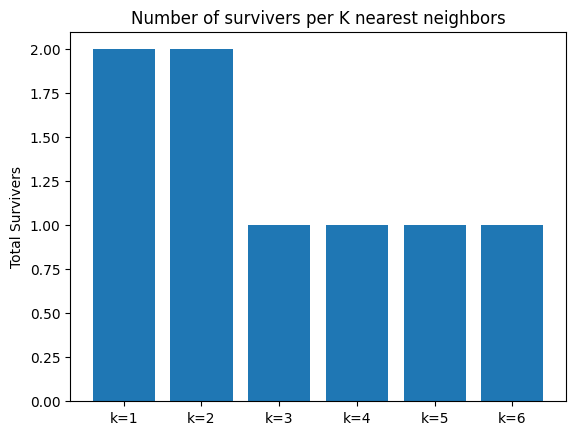
\includegraphics[scale=0.6]{bar_plot.png}}
    \item While $k=1$ and $k=2$ have the most survivors among my samples, I beleive that's because there isn't enough wiggle room for correct classification. I believe $k=6$ is most representative give the fact that I have 6 different features.
    \item The most apparent solution is to run multiple rounds of cross validation along different values for K to assess the accuracy.
  \end{enumerate}

\section*{Problem 5.2}
\begin{enumerate}[label=(\alph*)]
  \item
  \item
  \item
  \item
\end{enumerate}

\section*{Problem 5.3}

\section*{Problem 5.4}

\section*{Problem 5.5}

\end{document} 
































